\documentclass[11pt]{article}
\usepackage{../EllioStyle}
\usepackage{graphicx}

\title{Homework 5}
\author{Elliott Pryor \\
Collaborated with: Nathan Stouffer}
\date{25 March 2021}

\rhead{Homework 5}
\lhead{Elliott Pryor}

\graphicspath{{./}{images/}}




\makeatletter
\def\mathcolor#1#{\@mathcolor{#1}}
\def\@mathcolor#1#2#3{%
  \protect\leavevmode
  \begingroup
    \color#1{#2}#3%
  \endgroup
}
\makeatother


\algdef{SE}[DOWHILE]{Do}{doWhile}{\algorithmicdo}[1]{\algorithmicwhile\ #1}

\begin{document}

\maketitle


\problem{1}

In Homework 1, we considered a plane-sweep algorithm for determining whether
there is any intersection among a collection of $n$ circles in the plane. Here
we consider a variant of this problem. The input consists of a collection of $n$
closed circular disks, all having the same radius. (Via scaling, we may assume
that they are all unit disks.) Let $C = \{c_1, \ldots , c_n\}$ denote the center
points of these disks, and let $\{D_1, \ldots, D_n\}$ denote the actual disks.
Thus, $D_i$ consists of the points that lie within unit distance of $c_i$. Let
$U = D_1 \cup \ldots \cup D_n$ denote the union of these disks. The boundary of
$U$ may generally consist of multiple parts, each of which consists of a cycle
of circular arcs connected by vertices. (In Fig. 4 the boundary consists of
three cycles. The vertices are shown as white dots).

\begin{figure}[h]
    \centering
    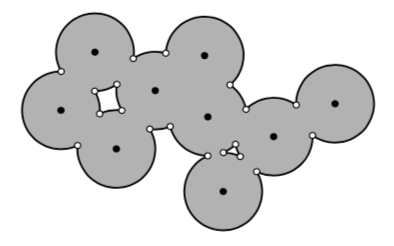
\includegraphics[width=0.4\textwidth]{union-of-disks}
    \caption{Problem 4: Union of disks}
\end{figure}

\begin{enumerate}

    \item Present an algorithm that reports all the vertices on the boundary of
        $U$. (Note that circle intersection points in the interior of the union
        are explicitly excluded.) Your algorithm should run in time $O(n log
        n)$.  The order in which the vertices are output is arbitrary. (Hint:
        Don't try to modify the algorithm from Homework 2. A different approach
        is needed.... think giraffes)

    \item Prove that the number of vertices reported by your algorithm is
        $O(n)$.

\end{enumerate}

\hrule





\begin{algorithm}[H]
    \caption{Verticies of Disks}
    \label{alg:neighbors}
    \begin{algorithmic}[1]
    \Function{disks}{$C$}
        \State Voronoi = Voronoi Diagram($C$)
        \State $P \gets []$
        \For{$c \in C$}
            \For{edge in Voronoi around cite $c$}
                \State if circle of radius 1 intersects edge, add it to $P$
            \EndFor
        \EndFor
        \State \textbf{return: } $P$
    \EndFunction
    \end{algorithmic}
\end{algorithm}


We assume that there are no isolated circles (or if there are we do not need to report them).
This could also be checked easily and still computed in $O(n \log n)$ if needed.
We also assume that the disks are closed, so if there is an intersection of 3 circles
at one point (vertex in voronoi) this does not count as hole in the union of disks.

\textbf{Runtime: }
This runs in $O(n \log n)$. We can compute the voronoi diagram (line 2)
using Fortune's algorithm on $O(n \log n)$. 
Then there are $n$ centers we look at in the first for loop.
From Euler's formula, we know that $|E| = O(n)$, that means around each center (face)
there are $O(1)$ edges. Thus the inner loop is $O(1)$ time (we can compute intersection in $O(1)$ time).

\textbf{Correctness: }
The correctness hinges on the following theorem,
a vertex is on the boundary iff the circle of radius 1 intersects the voronoi
edge belonging to the face in which the circle's center is the site. 

\begin{proof}
    We prove the reverse direction. 

    We first establish that if there is an intersection of circle and a voronoi edge,
    then there is an intersection of circles at that point. From the circle property,
    a point on a voronoi edge has a circle of some radius that touches 2 sites.
    Since there was an intersection of the edge with the circle, we know that the point is 
    exactly distance $R$ ($R=1$) from the first site, thus there must be another site at distance $R$
    from that point. Since all disks are of radius $R$, there is an intersection of the 2 disks at that point.

    We then show that this must be on the boundary (exterior). If the intersection occurs on a voronoi
    edge not belonging to this center, then the point on the voronoi edge is closer to 2 other sites,
    thus it is within them. So we only need to consider the voronoi edges belonging to the centers.

    Suppose that this intersection is in the interior. Then there must be another circle such that 
    the distance to the point is less than $R$ (1 in our case). 
    Then this point is not equidistant between our site and this other site. Thus it cannot be along the
    voronoi edge belonging to this site. A contradiction. Thus it must be exterior.
\end{proof}

We don't need to prove the forward direction for the correctness of the algorithm. 
So thus our algorithm does find the exterior intersections as required. 




\problem{2}

Suppose we are given a subdivision of the plane into $n$ convex regions. We
suspect that this subdivision is a Voronoi diagram, but we do not know the
sites. Develop an algorithm that finds a set of $n$ point sites whose Voronoi
diagram is exactly the given subdivision, if such a set exists.
\hrule

The challenging part of this problem is finding the first site.
Once we find the first site we can use the perpendicular bisector property of the edges to find the others.
As we do this, if we circle around and find conflicting information (a site should be in 2 different spots)
then we know it is not Voronoi. 

To find the first site, we need two vertices. If the graph has no vertices then a point anywhere works.
If it has 1 vertex, then we do the following to find the angles of the 3 sites. Then we place them 
at that angle at some common radius $R$.

We observe that if you reflect a site over the 3 edges around a vertex you get back to the original site.
We examine this vertex and edges in polar coordinates centered about the vertex.
Let the angle of the three lines be $\Theta_1, \Theta_2, \Theta_3$ listed in counter-clockwise order (clockwise order also works),
 and the angle of our site be $\phi$.
The first reflection is $\phi ' = \phi + 2(\Theta_1 - \phi)$ (shifts by double the angle gap between $\Theta_1$ and $\phi$)
This is more easily written as $\phi' = 2\Theta_1 - \phi$.
The second and third reflections follow similarly.

\begin{align}
    \phi ' &= \phi + 2(\Theta_1 - \phi) = 2\Theta_1 - \phi \\
    \phi '' &= \phi' + 2(\Theta_1 - \phi') = 2\Theta_1 - \phi'\\ 
    \phi ''' &= \phi'' + 2(\Theta_1 - \phi'') = 2\Theta_1 - \phi''
\end{align}

Since after the 3rd reflection it should come back to the same spot (after full rotation),
$\phi ''' = 2\pi + \phi$. We then substitute and solve this for $\phi$.

We get the surprisingly simple 
\begin{equation}
    \phi = (\Theta_3 - \Theta_2 + \Theta_1) - \pi
\end{equation}

Solving this equation around a vertex gives us the direction of a site. 

\textbf{Algorithm: }

find 2 adjacent vertices in the diagram, $v_1, v_2$. Solve for $\phi_1, \phi_2$ around each site.
We have that the shared edge on the first site is $\Theta_1$ and is $\Theta_3$ around the second site.
Our starting site is the intersection of the two lines through $v_1, v_2$ at angle $\phi_1, \phi_2$ 
respectively. 

\begin{figure}[h]
    \centering
    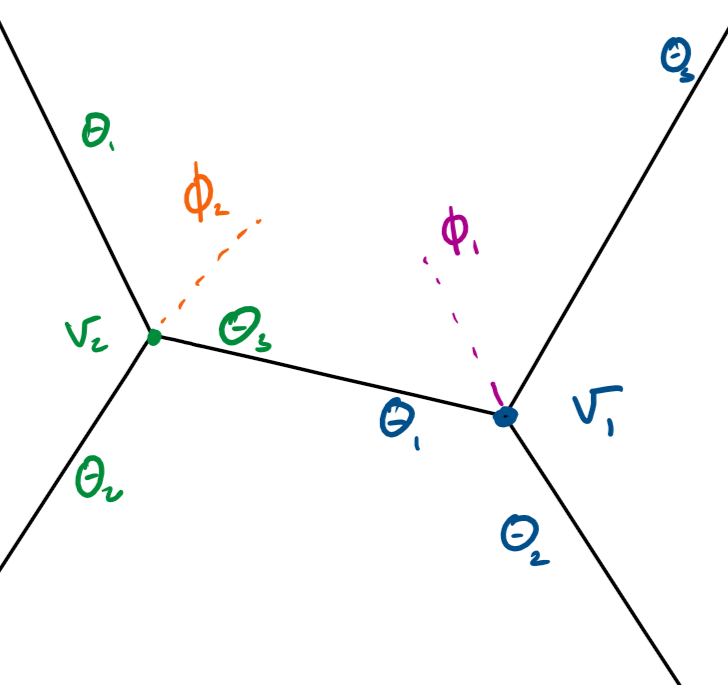
\includegraphics[width = 0.5\textwidth]{phi.png}
    \caption{Arrangement of $\Theta_1, \Theta_2, \Theta_3$ to solve for $\phi_1, \phi_2$}
\end{figure}

Then we do a breadth first search crossing each edge in the voronoi diagram. 
We compute the site across the edge by the perpendicular bisector property. 
Then we verify that this spot is the same as any previously computed site.
If there is a discrepancy, then return not voronoi.
Otherwise return the pointset computed. 


\textbf{Runtime: }

The first site can be computed in $O(1)$ time (solving 2 equations for $\phi_1, \phi_2$ and then line intersection)
Then the breadth first search traverses every edge in the voronoi diagram once. Since it is planar,
by Euler's formula we know that the number of edges is $O(n)$. So this algorithm works in $O(n)$.


\textbf{Correctness: }

As mentioned above there are a couple of weird edge cases that don't quite work.
If there is just 1 vertex (3 sites) this works we just choose $R > 0$ randomly.
We could have a set of just parallel lines (all sites co-linear). Where we just choose a perpendicular
line to this, and put a point in the middle of each segment. 
The nothing case which is trivial. 

But ignoring these edge cases, we show that it is correct. 
We established above that any point along $\phi$ is valid for a given voronoi vertex.
Any site must be consistent with all of its vertices. 
Clearly our chosen site is consistent with $v_1, v_2$, but what if it is inconsistent with another one.
Then, when we traverse an inconsistent edge, we will place a site at the wrong spot. 
When this wrong site is compared with another cell (ie it gets reflected across an edge)
it will be a different location then the site already there. So the algorithm will stop and return not voronoi
as required. 

\end{document}